\documentclass{standalone}
\usepackage{tikz}

\usepackage{color}

\usetikzlibrary{arrows.meta}
\usetikzlibrary{calc}
\usetikzlibrary{shapes}
\usetikzlibrary{bending}
\usetikzlibrary{patterns}

\usepackage{gensymb}

\usepackage{pgfplots}
\usepgfplotslibrary{polar}

\begin{document}
		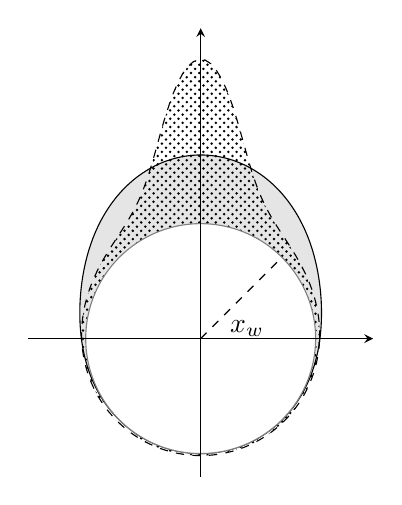
\begin{tikzpicture}[
	% scale=0.8,
	declare function={
		wc(\x) = 1 + 1/(2*pi)*(1-0.8*0.8)/(1+0.8*0.8-2*0.8*cos(deg(\x-0.5*pi))); %wc(mu=0.5pi, rho=0.5) 
		wn(\x)= 1 + 
		(1/sqrt(2*pi*0.446)*exp(-1/(2*0.446)*(\x-0.5*pi)*(\x-0.5*pi))) + (1/sqrt(2*pi*0.446)*exp(-1/(2*0.446)*(\x-2.5*pi)*(\x-2.5*pi))) +
		(1/sqrt(2*pi*0.446)*exp(-1/(2*0.446)*(\x+1.5*pi)*(\x+1.5*pi))); %wrappedN(mu=0.5pi, sd=2)
	}
	]	
	

	\begin{axis}[
	%scale=0.65,
	axis on top=true,
	unit vector ratio=1 1,
	axis x line=middle, axis y line=middle,
	xtick=\empty,
	ytick=\empty,
	xlabel=$x_w$,
	x label style={right=-16mm, above=-1mm},
	ymin=-1.2, ymax=2.7, 
	xmin=-1.5, xmax=1.5, 
	]
	
	\addplot[fill=white!90!black,data cs=polarrad, domain=0:2*pi,samples=300]{wn(x)};
	\addplot[dashed,pattern=crosshatch dots,data cs=polarrad, domain=0:2*pi,samples=300]{wc(x)};

	
	\addplot[samples=300, domain=0:2*pi,gray,fill=white]
	({cos(deg(x))}, {sin(deg(x))}) \closedcycle;
	
	%indication of angle
	\addplot[domain=0:0.5*1.41, dashed]{x};
	\end{axis}
	
	
	\end{tikzpicture}  
\end{document}